\section{A Brief Description of Autograd}
As part of a modern deep learning framework, we need to define functional units like
the one shown in \autoref{fig:ch2:block_form}. Not only must we be able to
calculate the forward evaluation of a block $Y=f(X,h)$ given an input $X$ and
(possibly) some learnable weights $h$, we must also be able to calculate the
passthrough and update gradients $\dLdx{X}$, $\dLdx{h}$ given $\dLdx{Y}$. This
typically involves saving $\dydx{Y}{X}$ and $\dydx{Y}{h}$ evaluated at the
current values of $X$ and $h$ when we calculate the forward pass.

For example, the simple ReLU: $Y = \F{max}(0,\ X)$, is not memory-less. On the
forward pass, we need to put a 1 in all the positions where $X > 0$, and a 0
elsewhere. For a convolutional layer, we need to save $X$ and $h$ to
correlate with $\dLdx{Y}$ on the backwards pass. It is up to the block designer
to manually calculate the gradients and design the most efficient way of
programming them.  
For clarity and repeatability, we give pseudocode for all the core operations
developed in our package \emph{PyTorch Wavelets}. 

\section{Fast Calculation of the DWT and IDWT}\label{sec:ch3:dwt}
To have a fast implementation of the Scattering Transform, we need a fast
implementation of the $\DTCWT$\@. Similarly, for a fast implementation of the $\DTCWT$ we
need a fast implementation of the DWT\@. Future work may also explore
the DWT as a basis for learning, so having an implementation that is fast and
can pass gradients through will prove beneficial in and of itself. 

\subsection{The Input}
Recall from \autoref{sec:ch2:conv_layers} that our input is a 3-D array with
channel dimension first, followed by the two spatial dimensions. For a minibatch
of images, this becomes a 4-D array, with the sample number in the first
dimension. I.e., for a minibatch of $N$ images with $C$ channels and $H\x W$ spatial support, the
input has shape: $N\x C\x H\x W$.

\subsection{Preliminary Notes}
There has been much research into the best way to do the DWT on a GPU, in
particular comparing the speed of Lifting \cite{sweldens_lifting_1998}, or
second-generation wavelets, to the direct convolutional methods.
\cite{tenllado_parallel_2008, galiano_improving_2011} are two notable such
publications, both of which find that the convolution-based implementations are
better suited for the massively parallel architecture found in modern GPUs. For
this reason, we implement a convolutional-based DWT.

As the DWT and IDWT use fixed filters, we do not need to calculate
$\dydx{L}{h}$ on the backwards pass. This means on the forward pass we
can save on memory by not storing $\dydx{Y}{h} = X$ (see
\autoref{sec:ch2:conv_grad}). We found it easiest to explicitly rewrite forward
and backward passes for the DWT, as the autograd mechanics would often
unnecessarily save intermediate activations.

For example, consider an input $X \in \reals[128\x 256\x 64\x 64]$. This is not
an unrealistically large input for a CNN, as often minibatch sizes are 128,
channels can be in the hundreds and $64\x 64$ pixels is a relatively common 
input size. If we were to represent these numbers as floats, it would require
512MB of space on a GPU (modern GPUs have about 10GB of memory, so this single
activation already requires 5\%). If we perform a DWT on this input, we would
require another 512MB of space for the output. Using naive autograd, PyTorch
(or another framework) saves an extra 512MB of memory for the backwards pass
to calculate $\dydx{L}{h}$, even if we specify it as not requiring a gradient.
This means we can save 50\% of the memory cost by being explicit about what is,
and what is not needed for backpropagation.

% Writing a DWT in low-level calls is not theoretically difficult to do.
% There are only a few things to be wary of. Firstly,
% We note that a `convolution' in most deep learning packages is in fact a correlation. This
% does not make any difference when learning filters but when using preset ones, as we
% want to do, it means that we must take care to reverse the filters beforehand.
% Secondly, the automatic
% differentiation will naturally save activations after every step in the DWT
% (e.g. after row filtering, downsampling and column filtering). This is for the
% calculation of the backwards pass. We do not need to save these intermediate
% activations as our filters are fixed and we can save memory by
% overwriting the automatic differentiation logic and defining our own backwards
% pass.


\subsection{Primitives}\label{sec:ch3:primitives}
\begin{figure}
  \centering
  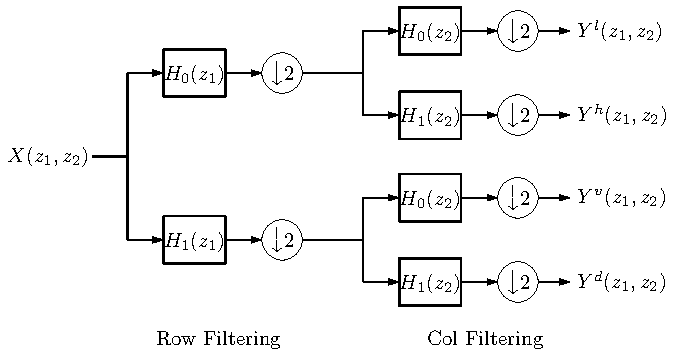
\includegraphics[width=0.8\textwidth]{\imgpath/dwt2d.pdf}
  \mycaption{2-D DWT filter bank layout}{The components of a filter bank DWT in
  two dimensions. $Y^l, Y^h, Y^v, Y^d$ represent the lowpass, horizontal,
  vertical, and diagonal components.}
  \label{fig:ch3:dwt}
\end{figure}

We start with the commonly known property that for a convolutional block, the
passthrough gradient is the gradient w.r.t.\ the output
convolved with the time reverse of the filter. More formally, if
$Y(z) = H(z) X(z)$, then:
%
\begin{equation}\label{eq:ch3:backprop}
  \Delta X(z) = H(z^{-1}) \Delta Y(z)
\end{equation}
%
where $H(z^{-1})$ is the $Z$-transform of the time/space reverse of $H(z)$,
$\Delta Y(z) \triangleq \dydx{L}{Y}(z)$ is the gradient of the loss with respect
to the output, and $\Delta X(z) \triangleq \dydx{L}{X}(z)$ is the gradient of
the loss w.r.t.\ the input. This was proved in \autoref{sec:ch2:conv_grad}, we
have just rewritten it in terms of $Z$-transforms here.

Additionally, for a decimation block, the passthrough gradient is
interpolation (see \autoref{sec:appB:samplegrads}
for a proof of this).

\autoref{fig:ch3:dwt} shows the block diagram for performing the forward pass of
a DWT\@. We can draw a similar figure for the backwards pass by replacing all the
forward operations with their passthrough gradients. Using the above two
properties, we see that the backwards pass of a DWT has the same form as
the inverse wavelet transform, with the time reverse of the analysis filters
used as the synthesis filters. For orthogonal wavelet transforms, the synthesis
filters are the time reverse of the analysis filters so backpropagation can be
done by doing the inverse wavelet transform with $\Delta Y^l(z), \Delta Y^h(z),
\Delta Y^v(z), \Delta Y^d(z)$. 
See \autoref{sec:appB:analysis_gradient} for more information on this
and the equivalent figure for the backwards pass.

{%
\renewcommand{\_}{\textscale{.8}{\textunderscore}}
Like Matlab, most deep learning frameworks have an
efficient function for doing convolution followed by downsampling. Similarly,
there is an efficient function to do upsampling followed by convolution (for the
inverse transform). Let us call these \texttt{conv2d\_down} and
\texttt{conv2d\_up} respectively\footnote{E.g.\ In PyTorch, convolution followed
by downsampling is done with a call to \texttt{torch.nn.functional.conv2d} with
the stride parameter set to 2.  Upsampling by 2 followed by convolution is done
by calling \texttt{torch.nn.functional.conv2d\_transpose}.}.
These functions, in turn, call the cuDNN low-level functions which can only support
zero padding or no padding (we called this \emph{valid convolution} in
\autoref{sec:ch2:padding}). If another padding type is desired, it must be done beforehand and 
valid convolution used.

With both \texttt{conv2d\_down} and \texttt{conv2d\_up}, we want to apply the
same filter to each channel of the input and \emph{not} sum them up (recall
\eqref{eq:ch2:conv4} sums over the channel dimension after doing convolution).
There are options available to prevent the summing in most frameworks, related
to doing \emph{grouped convolution}. For a good explanation on grouped
convolution, we recommend Chapter 5 of \cite{Ioannou2017thesis}. In our code
below, we assume that \texttt{conv2d\_down} and \texttt{conv2d\_up} act
independently on the $C$ channels and do not sum across them, giving an
output with the same shape as the input - $N\x C\x H\x W$.
}

\subsection{1-D Filter Banks}
Let us assume that the analysis ($h_0,\ h_1$) and synthesis ($g_0,\ g_1$)
filters are already in the form needed to do \emph{column} filtering. The necessary
steps to do the 1-D analysis and synthesis filtering are described in
\autoref{alg:ch3:fb1d}. We do not need to define backpropagation functions for the
\texttt{afb1d} (analysis filter bank 1-d) and \texttt{sfb1d} (synthesis filter
bank 1-D) functions as they are each other's backwards pass.

\begin{algorithm}[tb]
\caption{1-D analysis and synthesis stages of a DWT}\label{alg:ch3:fb1d}
\begin{algorithmic}[1]
  \label{alg:ch3:afb1d}
\Function{afb1d}{$x,\ h_0,\ h_1,\ mode,\ axis$}
  % \mbox{\\$h_0,\ h_1$ are 1-D lowpass and highpass filters}
  % \State $ h_0,\ h_1 \gets \F{flip}(h_0),\ \F{flip}(h_1) $\Comment{flip the filters for \texttt{conv2d_down}}
  \If{axis = 3}
    \State $h_0,\ h_1 \gets h_0^t,\ h_1^t$  \Comment{row filtering}
  \EndIf
  \State $p \gets \lfloor (\F{len}(x) + \F{len}(h_0) - 1) / 2 \rfloor$ \Comment{calculate output size}
  \State $b \gets \lfloor p/2 \rfloor$ \Comment{calculate pad size before}
  \State $a \gets \lceil p/2 \rceil$ \Comment{calculate pad size after}
  \State $x \gets \mathtt{pad}(x,\ b,\ a,\ mode)$ \Comment{pre pad the signal with selected mode}
  \State $lo \gets \mathtt{conv2d\_down} (x,\ h_0)$
  \State $hi \gets \mathtt{conv2d\_down} (x,\ h_1)$
  \State \textbf{return} $lo,\ hi$
\EndFunction
\end{algorithmic}\vspace{10pt}
\begin{algorithmic}[1]
  \label{alg:ch3:sfb1d}
\Function{sfb1d}{$lo,\ hi,\ g_0,\ g_1,\ axis$}
  % \mbox{\\$g_0,\ g_1$ are 1-D lowpass and highpass filters.}
  \If{axis = 3}
    \State $g_0,\ g_1 \gets g_0^t,\ g_1^t$  \Comment{row filtering}
  \EndIf
  \State $p \gets \F{len}(g_0) - 2$ \Comment{calculate output size}
  \State $lo \gets \mathtt{pad}(lo,\ p,\ p,\ `zero \textrm')$ \Comment{pre pad the signal with zeros}
  \State $hi \gets \mathtt{pad}(hi,\ p,\ p,\ `zero \textrm')$ \Comment{pre pad the signal with zeros}
  \State $x \gets \mathtt{conv2d\_up}(lo,\ g_0) + \mathtt{conv2d\_up}(hi,\ g_1)$
  \State \textbf{return} $x$
\EndFunction
\end{algorithmic}
\end{algorithm}

\subsection{2-D Transforms and Their Gradients}\label{sec:ch3:2d_dwt}
Having built the 1-D filter banks, we can easily generalize them to 2-D.
Furthermore, we can define the backwards steps of both the forward 2-D DWT
and the inverse 2-D DWT using these filter banks. We show how to do do this in
\autoref{alg:ch3:dwt}. The inverse transform logic is moved to the appendix - in
\autoref{alg:appB:idwt}.

Note that we have allowed for different row and column
filters in \autoref{alg:ch3:dwt}. Most commonly used wavelets will use the same
filter for both directions (e.g.\ the orthogonal Daubechies family), but later
when we use the $\DTCWT$, we will want to have different horizontal and vertical
filters.

Further, note that the only things that
need to be saved are the filters, as seen in
Algorithm~\algref{alg:ch3:dwt}{line:ch3:dwt_save}. These are typically only a
few floats, giving us a large saving over relying on autograd.

A multiscale DWT can easily be made by calling \autoref{alg:ch3:dwt}
multiple times on the lowpass output. Again, no intermediate activations need to be
saved, giving this implementation almost no memory overhead.

\begin{algorithm}[tb]
\caption{2-D DWT and its gradient}\label{alg:ch3:dwt}
\begin{algorithmic}[1]
\Function{DWT.Forward}{$x,\ h_0^r,\ h_1^r,\ h_0^c,\ h_1^c,\ mode$}
  \State \textbf{save} $h_0^r,\ h_1^r,\ h_0^c,\ h_1^c,\ mode$ \Comment{For the backwards pass} \label{line:ch3:dwt_save}
  \State $lo,\ hi \gets \mathtt{afb1d}(x,\ h_0^r,\ h_1^r,\ mode,\ axis=3)$ \Comment{row filter}
  \State $ll,\ lh \gets \mathtt{afb1d}(lo,\ h_0^c,\ h_1^c,\ mode,\ axis=2)$ \Comment{column filter}
  \State $hl,\ hh \gets \mathtt{afb1d}(hi,\ h_0^c,\ h_1^c,\ mode,\ axis=2)$ \Comment{column filter}
  \State \textbf{return} $ll,\ lh,\ hl,\ hh$
\EndFunction
\end{algorithmic}\vspace{10pt}
\begin{algorithmic}[1]
\Function{DWT.Backward}{$\Delta ll,\ \Delta lh,\ \Delta hl,\ \Delta hh$}
  \State \textbf{load} $h_0^r,\ h_1^r,\ h_0^c,\ h_1^c,\ mode$
  \State $\Delta lo \gets \mathtt{sfb1d}(\Delta ll,\ \Delta lh,\ h_0^c,\ h_1^c,\ mode,\ axis=2) $
  \State $\Delta hi \gets \mathtt{sfb1d}(\Delta hl,\ \Delta hh,\ h_0^c,\ h_1^c,\ mode,\ axis=2) $
  \State $\Delta x \gets \mathtt{sfb1d}(\Delta lo,\ \Delta hi,\ h_0^r,\ h_1^r,\ mode,\ axis=3) $
  \State \textbf{return} $\Delta x$
\EndFunction
\end{algorithmic}
\end{algorithm}

\section{Fast Calculation of the $\DTCWT$}\label{sec:ch3:dtcwt}
\begin{figure}
  % 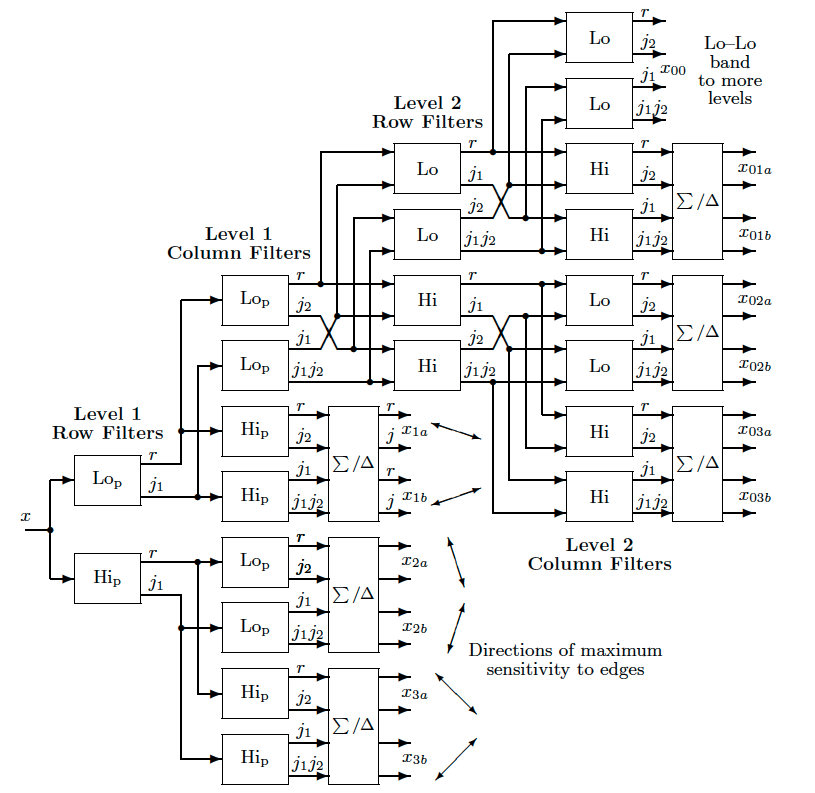
\includegraphics[width=\textwidth]{\imgpath/dtcwt_fb.png}
  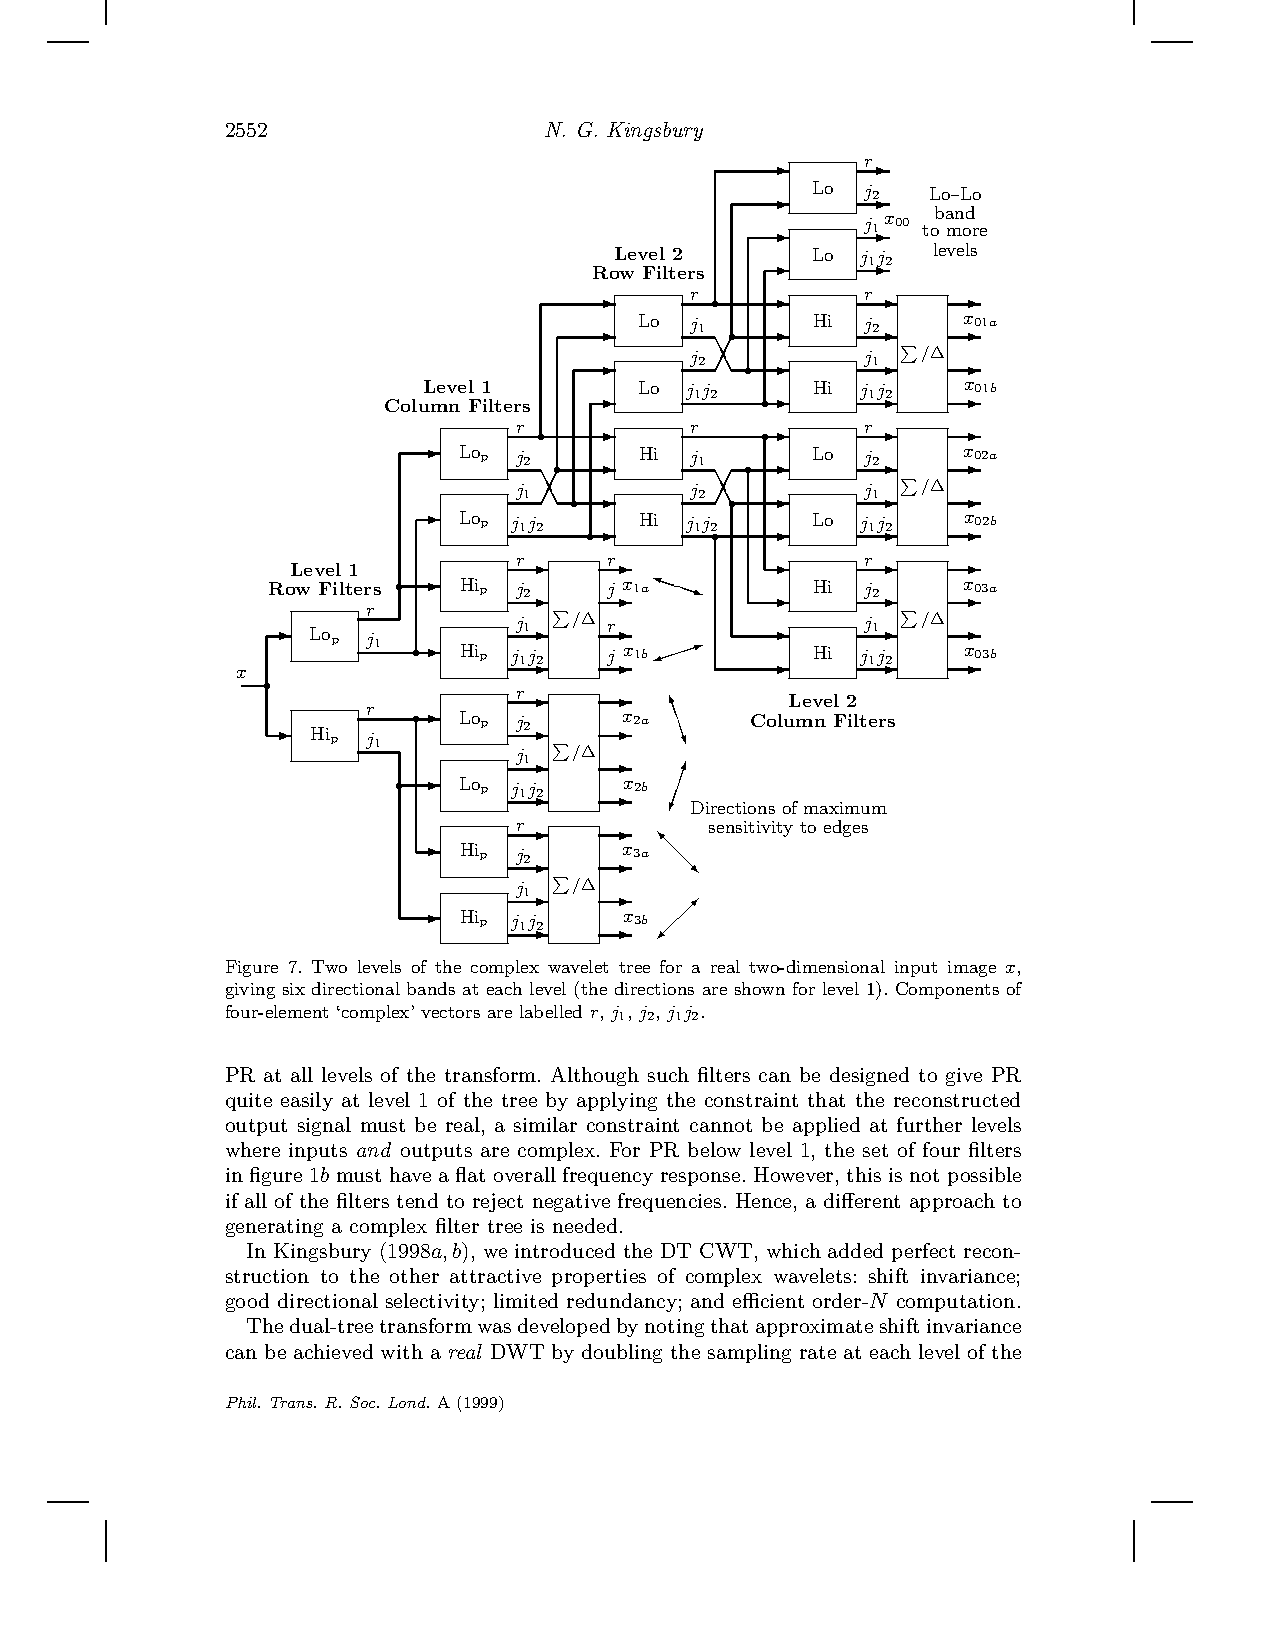
\includegraphics[trim=3cm 11.8cm 4cm 2.5cm, clip, width=\textwidth]{\imgpath/dtcwt_fb2}
  \mycaption{2-D $\DTCWT$ filter bank layout}{Two levels of the complex wavelet tree
  for a real 2-D input image $x$. The four DWTs involved in the $\DTCWT$ are
  labelled with $r$, $j_1$, $j_2$ and $j_1j_2$. Image is taken from \cite{kingsbury_image_1999}.}
  \label{fig:ch3:dtcwt_fb}
\end{figure}
We have built upon previous implementations of the $\DTCWT$
\cite{kingsbury_dtcwt_2003, cai_2-d_2011, wareham_dtcwt_2014}. The `dual-tree'
part of the $\DTCWT$ comes from it having two trees, each with their own set of filters:
$a = \{h_0^a, h_1^a, g_0^a, g_1^a\}$ and $b = \{h_0^b, h_1^b, g_0^b, g_1^b\}$. In one dimension, this
can be done with two DWTs, one using the $a$ filters and the other using the $b$
filters. In two dimensions, we must instead do
four multiscale DWTs. We follow the notation in \cite{kingsbury_image_1999} and
maintain separate imaginary operators $j_1$ and $j_2$ for the row and column
processing. We call our four DWTs $r,\ j_1,\ j_2,\ j_1j_2$ and show how the
filter bank system is connected in \autoref{fig:ch3:dtcwt_fb}. The output of
these four DWTs can be interpreted as a four-element `complex' vector $\{a, b,
c, d\} = a + bj_1 + cj_2 + dj_1j_2$. This 4-vector can be converted into a pair
of complex 2-vectors by letting $j_1 = j_2 = j$ in one case and $j_1 = -j_2=-j$
in the other case, producing the two outputs:
\begin{align}
  (a-d) + (b+c)j\\
  (a+d) + (-b+c)j
\end{align}
corresponding to the first and second quadrant directional filters respectively.
The sum and difference blocks $\Sigma/\Delta$ in \autoref{fig:ch3:dtcwt_fb} do
this operation \cite{kingsbury_image_1999}. 

The four lowpass coefficients from each scale are used for the next scale DWTs. At the
final scale, they are interleaved to get four times the expected lowpass output
area expected from a single decimated DWT\@.
See \autoref{alg:ch3:dtcwt} for the code on how to do the full $\DTCWT$.

A requirement of the $\DTCWT$ is the need to use different filters for the first
scale to all subsequent scales \cite{selesnick_dual-tree_2005}. We have not
shown this in \autoref{alg:ch3:dtcwt} for simplicity, but it would simply mean
we would have to handle the $j=1$ case separately.

We have moved the inverse $\DTCWT$ algorithm to \autoref{alg:appB:idtcwt}. Note
that for both the $\DTCWT$ and inverse $\DTCWT$, we rely on autograd to
calculate the backwards pass by calling our defined DWT.Forward and 
DWT.Backward methods.

\begin{algorithm}[t]
\caption{2-D $\DTCWT$. }\label{alg:ch3:dtcwt}
\begin{algorithmic}[1]
\Function{DTCWT}{$x,\ J,\ mode$}
\State \textbf{load} $h_0^a,\ h_1^a,\ h_0^b,\ h_1^b$ \Comment{Load from memory}
\State $ll_{r},\ ll_{j_1},\ ll_{j_2},\ ll_{j_1j_2} \gets x/2$
% \State $H = \left[h_
\For{$1 \le j \le J$}
\State $ll_{r},\ lh_{r},\ hl_{r},\ hh_{r} \gets \F{DWT}_{r}(ll_{r},\ h_0^a,\ h_1^a,\ h_0^a,\ h_1^a,\ mode)$
\State $ll_{j_1},\ lh_{j_1},\ hl_{j_1},\ hh_{j_1} \gets \F{DWT}_{j_1}(ll_{j_1},\ h_0^b,\ h_1^b,\ h_0^a,\ h_1^a,\ mode)$
\State $ll_{j_2},\ lh_{j_2},\ hl_{j_2},\ hh_{j_2} \gets \F{DWT}_{j_2}(ll_{j_2},\ h_0^a,\ h_1^a,\ h_0^b,\ h_1^b,\ mode)$
\State $ll_{j_1j_2},\ lh_{j_1j_2},\ hl_{j_1j_2},\ hh_{j_1j_2} \gets \F{DWT}_{j_1j_2}(ll_{j_1j_2},\ h_0^b,\ h_1^b,\ h_0^b,\ h_1^b,\ mode)$
  % \State \begin{varwidth}[t]{\linewidth}
    % $yh[j] \gets \F{Q2C}( $\par
        % \hskip\algorithmicindent $lh_{r},\ hl_{r},\ hh_{r},$ \par
        % \hskip\algorithmicindent $lh_{j_1},\ hl_{j_1},\ hh_{j_1},$ \par
        % \hskip\algorithmicindent $lh_{j_2},\ hl_{j_2},\ hh_{j_2},$ \par
        % \hskip\algorithmicindent $lh_{j_1j_2},\ hl_{j_1j_2},\ hh_{j_1j_2})$
        % \end{varwidth}
  \State $x_{1a} \gets (lh_{r} - lh_{j_1j_2}) + j(lh_{j_1} + lh_{j_2}) $ 
  \State $x_{1b} \gets (lh_{r} + lh_{j_1j_2}) + j(-lh_{j_1} + lh_{j_2}) $ 
  \State $x_{2a} \gets (hl_{r} - hl_{j_1j_2}) + j(hl_{j_1} + hl_{j_2}) $ 
  \State $x_{2b} \gets (hl_{r} + hl_{j_1j_2}) + j(-hl_{j_1} + hl_{j_2}) $ 
  \State $x_{3a} \gets (hh_{r} - hh_{j_1j_2}) + j(hh_{j_1} + hh_{j_2}) $ 
  \State $x_{3b} \gets (hh_{r} + hh_{j_1j_2}) + j(-hh_{j_1} + hh_{j_2}) $ 
  \State $yh[j] \gets (x_{1b},x_{3b}, x_{2b}, x_{2a}, x_{3a}, x_{1a}) $
\EndFor
\State $yl \gets \F{interleave}(ll_{r},\ ll_{j_1},\ ll_{j_2},\ ll_{j_1j_2})$
\State \textbf{return} $yl,\ yh$
\EndFunction
\end{algorithmic}
\end{algorithm}

\section{The $\DTCWT$ ScatterNet}\label{sec:ch3:scat}
\subsection{The Magnitude Operation}\label{sec:ch3:mag}

\begin{algorithm}[tb]
\caption{Magnitude forward and backward steps}\label{alg:ch3:mag}
\begin{algorithmic}[1]
\Function{MAG.Forward}{$x,\ y$}
  \State $r \gets \sqrt{x^2 + y^2}$
  \State $\theta \gets \arctan2(y,\ x)$ \Comment{$\arctan2$ handles $x=0$}
  \State \textbf{save} $\theta$
  \State \textbf{return} $r$
\EndFunction
\end{algorithmic}\vspace{10pt}
\begin{algorithmic}[1]
\Function{MAG.Backward}{$\Delta r$}
  \State \textbf{load} $\theta$
  \State $\Delta x \gets \Delta r \cos{\theta}$ \Comment{Reinsert phase}
  \State $\Delta y \gets \Delta r \sin{\theta}$ \Comment{Reinsert phase}
  \State \textbf{return} $\Delta x,\ \Delta y$
\EndFunction
\end{algorithmic}
\end{algorithm}
Now that we have a forward and backward pass for the $\DTCWT$, the final missing
piece is the magnitude operation. If $z = x + jy$, then:
%
\begin{equation}
  r = |z| =  \sqrt{x^2 + y^2}
\end{equation}
%
This has two partial derivatives, $\dydx{r}{x},\ \dydx{r}{y}$:
\begin{align}
  \dydx{r}{x} & =  \frac{x}{\sqrt{x^2 + y^2}} = \frac{x}{r}\\
  \dydx{r}{y} & =  \frac{y}{\sqrt{x^2 + y^2}} = \frac{y}{r}
\end{align}
Given an input gradient, $\Delta r$, the passthrough gradient is:
\begin{eqnarray}
  \Delta z & = & \Delta r \dydx{r}{x} + j\Delta r \dydx{r}{y} \\
           &= & \Delta r \frac{x}{r} + j\Delta r \frac{y}{r} \\
           &=& \Delta r e^{j\theta}
\end{eqnarray}
where $\theta = \arctan{\frac{y}{x}}$. This has a nice interpretation to it as
well, as the backwards pass is simply reinserting the discarded phase
information. The pseudocode for this operation is shown in
\autoref{alg:ch3:mag}.
%
These partial derivatives are restricted to be in the range $[-1, 1]$ but have a singularity at the origin.
In particular:
\begin{align}
  \lim_{x\rightarrow 0^{-},y\rightarrow 0}  \dydx{r}{x} &= -1 \\
  \lim_{x\rightarrow 0^{+},y\rightarrow 0}  \dydx{r}{x} &= +1 \\
  \lim_{x\rightarrow 0,y\rightarrow 0^{-}}  \dydx{r}{y} &= -1 \\
  \lim_{x\rightarrow 0,y\rightarrow 0^{+}}  \dydx{r}{y} &= +1
\end{align}
Rather than using the subgradient method \cite{boyd_subgradient_2003} which is
commonly used to handle the magnitude operation, we propose to smooth the
magnitude operator:
% These partial derivatives are very rapidly varying around 0 and the second
% derivatives go to infinity at the origin. This is not a
% feature commonly seen with other nonlinearities such as the tanh and sigmoid
% but it is seen with the ReLU. Small changes in the input can cause large changes
% in the propagated gradients.
% The bounded nature of the first derivative somewhat restricts the impact of
% possible problems so
% long as our optimizer does not use higher order derivatives (this is commonly
% Nonetheless, we propose to slightly smooth the magnitude operator:

\begin{equation}\label{eq:ch3:magbias}
 r_s = \sqrt{x^2 + y^2 + b^2} - b
\end{equation}

This keeps the magnitude near zero for small $x,y$ but does slightly shrink larger
values, however, our gradient is smoother and we no
longer have to worry about dividing by zero issues when calculating gradients.
% \textbf{Plot this}
We can choose the size of $b$ as a hyperparameter in optimization, which we
revisit in \autoref{sec:ch3:dtcwt_hypes}. The partial derivatives now become:
\begin{eqnarray}
  \dydx{r_s}{x} & = & \frac{x}{\sqrt{x^2 + y^2+b^2}} = \frac{x}{r_s}\\
  \dydx{r_s}{y} & = & \frac{y}{\sqrt{x^2 + y^2+b^2}} = \frac{y}{r_s}
\end{eqnarray}
There is a memory cost associated with this, as we will now need to save both
$\dydx{r_s}{x}$ and $\dydx{r_s}{y}$ as opposed to saving only the phase.
\autoref{alg:appB:mag_smooth} has the pseudocode for the smooth magnitude.

\subsection{Putting it all Together}\label{sec:ch3:combining}

\begin{algorithm}[tb]
  \caption{$\DTCWT$ ScatterNet Layer}
  \label{alg:ch3:dtcwt_scat}
\begin{algorithmic}[1]
\Function{DTCWT\_SCAT}{$x,\ J=2,\ M=2$}
\State $Z \gets x$
\For{$1 \le m \le M$}
  \State $yl,\ yh \gets \DTCWT(Z,\ J=1,\ mode=\F{`symmetric \textrm'})$
  \State $S \gets \F{avg\_pool}(yl,\ 2)$
  \State $U \gets \F{mag}(\real{yh},\ \imag{yh})$
  \State $Z \gets \F{concatenate}(S,\ U,\ axis=1)$ \Comment{stack 1 lowpass with 6 magnitudes}
\EndFor
\If{$J > M$}
\State $Z \gets \F{avg\_pool}(Z,\ 2^{J-M})$
\EndIf
\State \textbf{return} $Z$
\EndFunction
\end{algorithmic}
\end{algorithm}
Now that we have the $\DTCWT$ and the magnitude operation, it is straightforward
to get a $\DTCWT$ scattering layer, shown in \autoref{alg:ch3:dtcwt_scat}.

For a second-order ScatterNet, the first $C$ channels of $Z$ from
\autoref{alg:ch3:dtcwt_scat} are the $S_0$ coefficients, the next $JKC$ are the
$S_1$ coefficients and the final $\frac{1}{2}(J-1)JK^2C$ channels are the
$S_2$ coefficients.

For ease in handling the different sample rates of the lowpass and the
bandpass, we have averaged the lowpass over a $2\x 2$ window and downsampled it
by 2 in each direction. This slightly
affects the higher-order scattering coefficients, as the true $\DTCWT$ needs the doubly
sampled lowpass for the second scale, however, we noticed little difference in
performance from doing the true $\DTCWT$ and this slightly modified one

\subsection{$\DTCWT$ ScatterNet Hyperparameter Choice}\label{sec:ch3:dtcwt_hypes}
{%
\renewcommand{\_}{\textscale{.6}{\textunderscore}}
\begin{table}[bt]
  \centering
  \mycaption{Hyperparameter settings for the $\DTCWT$ ScatterNet}{}
  \label{tab:ch3:hyper_options}
  \begin{tabular}{l l l}
    \toprule
    Hyperparameter & \hphantom{ab} & Values \\
    \midrule
    Wavelet && \multicolumn{1}{l}{near\_sym\_a 5,7 tap filters} \\
            && \multicolumn{1}{l}{near\_sym\_b 13,19 tap filters}\\
            && \multicolumn{1}{l}{near\_sym\_b\_bp 13,19 tap filters} \\\midrule
    Padding Scheme && symmetric \\
                   && zero  \\\midrule
    Magnitude Smoothing $b$ && 0 \\
                            && 1e-3 \\
                            && 1e-2 \\
                            && 1e-1
    \\\bottomrule
  \end{tabular}
\end{table}
Before comparing to the Morlet-based ScatterNet, we test
different padding schemes, wavelet lengths and magnitude smoothing parameters (see
\eqref{eq:ch3:magbias}) for the $\DTCWT$ ScatterNet. We test these over a grid of values described in
\autoref{tab:ch3:hyper_options}. 

The different wavelets have different lengths
and hence different frequency responses. Additionally, the `near\_sym\_b\_bp'
wavelet is a rotationally symmetric wavelet with diagonal passband brought in by
a factor of $\sqrt{2}$, making it have similar $|\bm{\omega}|$ to the horizontal
and vertical bandpasses.

The results of these experiments are shown in \autoref{fig:ch3:hypes}.
The choice of options can have a significant impact on 
classification accuracy. Symmetric padding appears to work marginally better than zero padding.
Surprisingly, the shorter filters (near\_sym\_a) fare better than their longer counterparts
and bringing in the diagonal subbands (near\_sym\_b\_bp) does not help.
Additionally, the smoothing bias may indeed be a good idea for the forward
pass as well as aiding the backwards pass, so long as it is less than 0.1.

However, it is difficult to tell just how much `better' the different filter lengths and
padding schemes are, as there are many other factors to take into
consideration when training a CNN\@. The standard deviations for the results from
\autoref{fig:ch3:hypes} were all in the range from 0.1 to 0.4\% for the two CIFAR
datasets, which is smaller
than the 2\% range seen from the best option to the worst. However, for
the larger Tiny ImageNet dataset the standard deviations were in the range from 0.2 to 0.6\%,
which is comparable to the 1\% difference between the `best' and `worst' configurations.

We proceed by using the `near\_sym\_a' filters, with symmetric padding and a
smoothing factor of 0.01, but leave all configurations in our code in \cite{cotter_pytorch_2018}
and note that more experimentation needs to be done in analysing and comparing the
choice of options.

\begin{figure}[h!]
  \subfloat[CIFAR-10]{%
    \hspace{-1.2cm}
    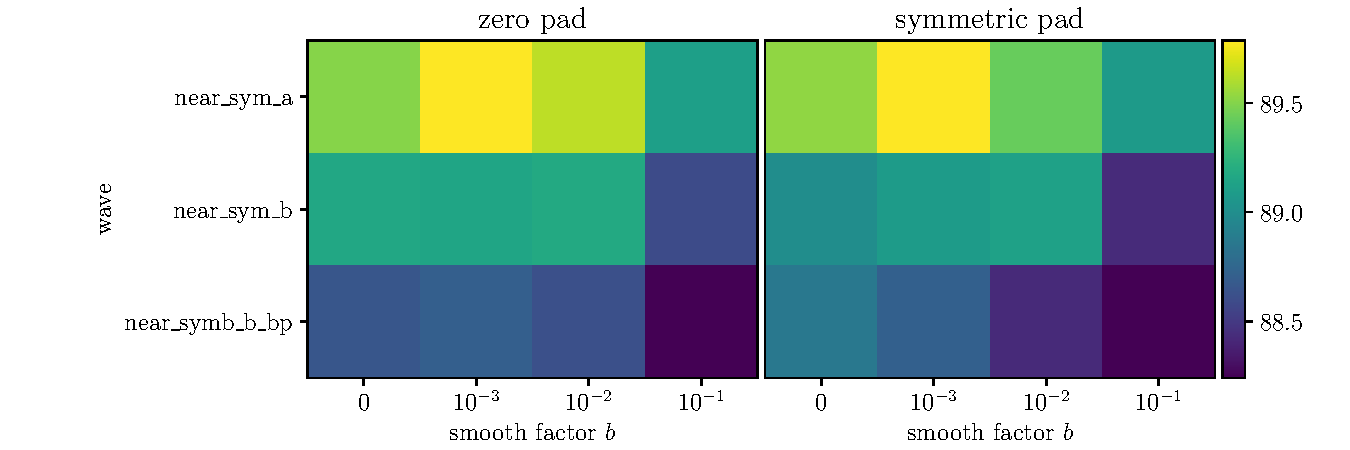
\includegraphics[width=\textwidth,height=5cm]{\imgpath/cifar10_scat_options.pdf}
    \label{fig:ch3:hypes_cifar10}
    }
    \vspace{-0.3cm}
    \\
  \subfloat[CIFAR-100]{%
    \hspace{-1.2cm}
    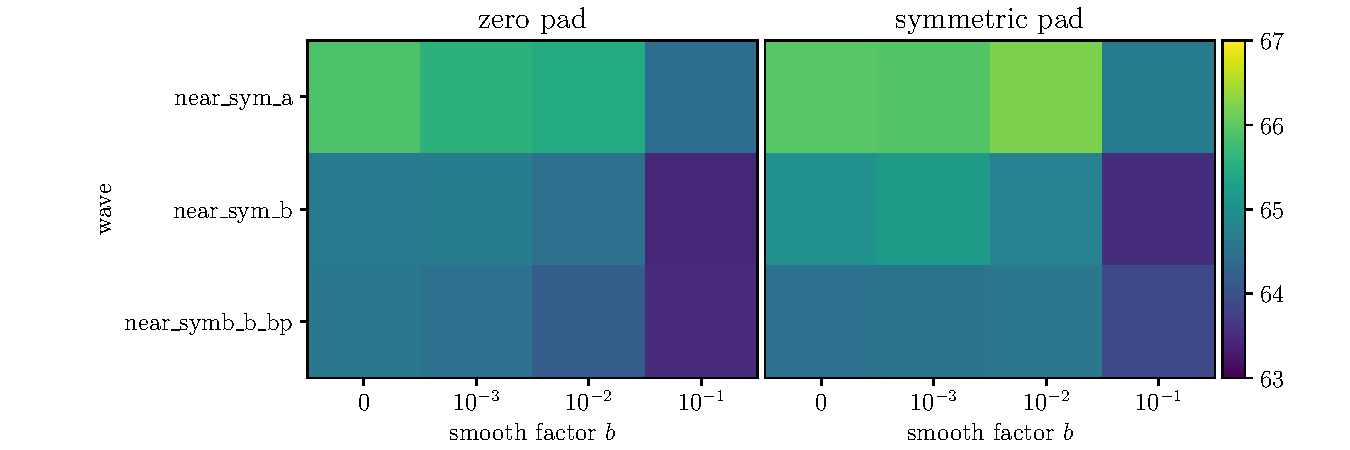
\includegraphics[width=\textwidth,height=5cm]{\imgpath/cifar100_scat_options.pdf}
    \label{fig:ch3:hypes_cifar100}
    }
    \vspace{-0.3cm}
    \\
  \subfloat[Tiny ImageNet]{%
    \hspace{-1.2cm}
    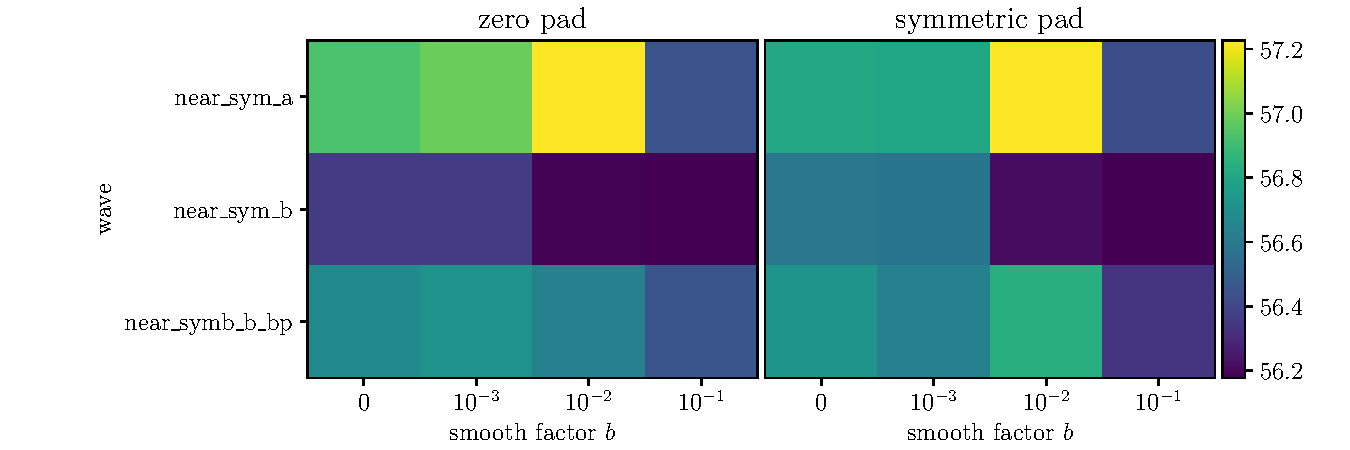
\includegraphics[width=\textwidth,height=5cm]{\imgpath/ti_scat_options.pdf}
    \label{fig:ch3:hypes_ti}
    }
    \vspace{-0.2cm}
    % \mycaption{}{}
 \mycaption{Hyperparameter results for the $\DTCWT$ ScatterNet on various
  datasets}{Image showing relative top-1 accuracies (in \%) on the given datasets using
  architecture described in \autoref{tab:ch3:hyper_options}. Each subfigure is a new
  dataset and therefore has a new colour range (shown on the right). Results are
  averaged over 3 runs from different starting positions.
  The choice of options can have a very large impact on
  classification accuracy. Symmetric padding is marginally better than zero padding.
  Surprisingly, the shorter filter (near\_sym\_a) fares better than its longer counterparts,
  and bringing in the diagonal subbands (near\_sym\_b\_bp) does not help.
  Additionally, the smoothing bias may indeed be a good idea for the forward
  pass as well as aiding the backwards pass, so long as it is less than 0.1.}
  \label{fig:ch3:hypes}
\end{figure}

}
% \newpage
